\documentclass[twocolumn]{aastex61}
\usepackage{natbib}
\bibliographystyle{apj}
\usepackage{graphicx}
\usepackage{amsmath}

\newcommand{\citeth}[1]{(\citeauthor{#1}\ \citeyear{#1})}
\newcommand{\citethnop}[1]{\citeauthor{#1}\ \citeyear{#1}}
\newcommand{\citethnopp}[1]{\citeauthor{#1}\ (\citeyear{#1})}



\def \lya {Ly$\alpha$ }
\def \mkms {{\rm \; km\;s^{-1}}}
\def \msunperyr {{\; M_{\odot}\rm \;yr^{-1}}}

\begin{document}
\title{A VLT/FORS2 Narrowband Imaging Search for \ion{Mg}{2} Emission Around $\lowercase{z}\sim0.7$ Galaxies }
\author{Ryan Rickards Vaught}
\affiliation{Department of Astronomy, San Diego State University, San Diego, CA 92182}
\affiliation{Department of Physics, University of California, San Diego, 9500 Gilman Dr. La Jolla, CA 92093, USA} 
 
 \author{Kate H. R. Rubin }
 \affiliation{Department of Astronomy, San Diego State University, San Diego, CA 92182, USA}
 
 \author{Fabrizio Arrigoni Battaia }
 \affiliation{European Southern Observatory, Karl-Schwarzschild-Str. 2, D-85748 Garching bei M\"unchen, Germany}

 \author{J. Xavier Prochaska}
 \affiliation{Astronomy \& Astrophysics, UC Santa Cruz, 1156 High St., Santa Cruz, CA 95064 USA}
 
\author{Joseph F. Hennawi}
\affiliation{Department of Physics, Broida Hall, University of California, Santa Barbara, CA 93106-9530}

\correspondingauthor{Ryan Rickards Vaught}
\email{rjrickar@ucsd.edu}

\begin{abstract}

The mass and energy of galactic winds remain poorly constrained via QSO and ``down-the-barrel" absorption line studies. One way to better constrain these parameters is to measure the spatial extent of the outflow in emission. We perform a VLT/FORS2 narrowband imaging search around 5 star-forming galaxies at redshift $z=0.67-0.69$ in the Great Observatories Origins Deep Survey South (GOODS-S) field to constrain the radial extent of large-scale outflows traced by resonantly scattered \ion{Mg}{2} emission. These observations probe unmatched surface brightness limits of 5.74 $\times$ $10^{-19}$ ergs sec $^{-1}$ cm$^{-2}$ arcsec$^2$ (5$\sigma$).  We do not detect any extended emission around any of the sample galaxies, thus placing strong upper limits on the brightness of \ion{Mg}{2} emission at projected distances $R_{\perp} = 13-24$ kpc. The imaging also resolves the \ion{Mg}{2} observed galaxy spatially, revealing approximately constant absorption strengths across the galaxy disks. Our detection limits in concert with a previous studies Keck/LRIS spectra allow us to compare our observations to previous radiative transfer models of \ion{Mg}{2} emission for isotropic and anisotropic dust/dust-free winds. Based on these comparisons, if our galaxies do host \ion{Mg}{2} emission, then the predicted \ion{Mg}{2} based on this modeling suggests that these winds are anisotropic and dusty for any scattered \ion{Mg}{2} emission to lie below our 5$\sigma$ detection limits.

\end{abstract}

\keywords{galaxies: evolution, galaxies: absorption lines}

\section{Introduction}\label{sec:intro}
Galactic winds play a critical role in regulating the star formation rates and stellar masses of galaxies \citeth{Werk_2014}; however, the physics that powers these winds remains uncertain. Some possible mechanisms have been proposed by theoretical studies that include thermal pressure from core collapse supernovae, radiation pressure from starbursts, and finally cosmic ray pressure (\citethnop{Larson_1974}; \citethnop{Chevalier_1985}; \citethnop{Springel_2003}; \citethnop{Sugahara_2017}). Additionally, the impact galactic winds have on their host galaxies (i.e., their mass and energy content) has remained difficult to constrain with observations.

An accurate picture of the types of galaxies that host outflows comes from numerous absorption line studies of galaxies (\citethnop{Veilleux2005}; \citethnop{Weiner2009}; \citethnop{Martin2012}; \citethnop{Rubin_2014}). Gas flows are detected by measuring the blueshift (outflow) or redshift (inflow) of absorption transitions with respect to the host galaxy systemic velocity. Spectroscopy of galaxies from low to high redshifts probing cold gas ($T \lesssim 10^2$ K) which absorbs in \ion{Na}{1} and cool gas ($T \sim 10^4$ K) in \ion{Mg}{2} has revealed outflows in most galaxies that host active star-formation (e.g. \citethnop{chen2010}; \citethnop{Martin2012}; \citethnop{Rubin_2014}).
Even though this technique constrains the radial velocity, column density and covering fraction of the flow, it weakly constrains the overall radial extent and provides no information on the morphology of the gas.

An alternative method that can in principal asses the radial extent and morphology of outflows is to trace the gas in emission. This has been demonstrated using rest-frame optical transitions (i.e H$\alpha$, [\ion{O}{3}], etc) as tracers for winds around nearby starbursts \citep[][]{{Matsubayashi2009,Veilleux2009}} as these transitions can trace the warm shock heated phase of the gas. 
Another transition potentially useful for tracing winds in emission is the \ion{Mg}{2} $\lambda\lambda 2976,2803$ doublet in the rest-frame ultraviolet
\citep[UV;][]{{Weiner2009, Kornei2013}}. While most studies of winds using \ion{Mg}{2} have focused on its absorption kinematics, \cite{Rubin_2011} observed  strong \ion{Mg}{2} emission with a P-Cygni line profile in the spectrum of a strongly star-forming galaxy at redshift $z = 0.694$. In addition, the emission was spatially extended, permitting the first direct measurement of the extent of an outflow ($>$ 7 kpc) in the distant universe.

One proposed production mechanism for such P-Cygni profiles is photon scattering. In this mechanism, \ion{Mg}{2} ions in the region of the wind closest to the observer will absorb continuum photons in the resonant transitions at wavelengths 2796\AA, $\lambda_{2796}$, and 2803, \AA $\lambda_{2803}$. Once these transitions are excited, they may only decay back to the ground state. If the optical depth of the gas is high, then the gas will resonantly trap the absorbed photons. Because the photons are absorbed in the rest frame of the gas, the absorption will be blueshifted relative to the galaxy's systemic velocity. The \ion{Mg}{2} ions in the section of the wind farthest from the observer will absorb and scatter photons that are redshifted relative to the front portion of the wind. Because the photons are redshifted, the photons travel freely towards the observer through the wind to produce emission at and redward of the systemic velocity of the galaxy (\citethnop{Rubin_2011}, \citethnop{Prochaska_2011}). Since the first detection of \ion{Mg}{2} emission in an individual galaxy by \citet{Rubin_2011}, another detection was reported by \cite{Martin2013}, who observed \ion{Mg}{2} emission that extends $12-18$ kpc from a strongly star-forming galaxy
at $z=0.9392$. \ion{Mg}{2} has also been studied in wide-field galaxy surveys conducted with Keck/DEIMOS and VLT/MUSE  (\citethnop{Weiner2009}, \citethnop{Kornei2013},\citethnop{Erb2012}, \citethnop{Feltre2018}). These surveys, which include galaxies with redshifts $ 0.70 < z < 2.30$, find that \ion{Mg}{2} may be detected in pure emission, pure absorption or with P-Cygni profiles and that detections of \ion{Mg}{2} in emission were found to be associated with galaxies of lower stellar mass and bluer spectral slopes.

The diversity of these spectral profiles may be understood using radiative transfer modeling of galactic winds.
\citet{Prochaska_2011} have used this technique to predict 
spectra for the  \ion{Mg}{2} and  \ion{Fe}{2}$^*$ fine-structure transitions for a variety of wind morphologies.
The authors demonstrated that isotropic dust-free winds will conserve photon flux, thus predicting that blueshifted absorption lines should be accompanied by emission lines with similar equivalent widths (EW). Anisotropic winds, however, were demonstrated to exhibit significantly weaker emission by a factor proportional to the angular extent (i.e., solid angle) of the wind. Scattered emission was found to be additionally weakened by the inclusion of dust and the presence of a strongly-absorbing interstellar medium (ISM).
Thus, spatially-resolved measurement of the surface brightness of this emission constrains not only the radial extent of the emitting material, but also its morphology and dust content.

In this paper, we present the first narrowband imaging of the \ion{Mg}{2} transition around 5 star-forming  galaxies located in the  GOODS-S field at redshift $z \sim 0.7$. 
We use two filters: a  ``line filter" covering the \ion{Mg}{2} doublet, and a ``continuum filter" that is offset from the line filter by ${\sim}47$ \AA.    
The resulting imaging in each filter has a total integration time of 10 hrs. As opposed to 1D spectra, the narrowband imaging constrains the surface brightness, optical depth and radial extent of the wind. These observations allow us to create the first ever high-S/N spatially resolved map of both \ion{Mg}{2} emission and absorption. 

In Section \ref{sec:obs_red} we describe our sample of GOOD-S galaxies, supplemental Keck/LRIS spectra, as well as our VLT/FORS2 observations, image reduction, and absolute flux calibration. We describe our method of continuum subtraction in Section \ref{sec.cont_sub}. Analysis of these data is presented in Section \ref{sec:analysis}, 
including our methods for calculating surface brightness profiles and detection limits for each galaxy, as well as maps of \ion{Mg}{2} equivalent widths.
Section \ref{sec:results} presents results from this analysis. We compare our SB detection limits to previous detections of extended \ion{Mg}{2} emission,  and compare our observations to predictions made by radiative transfer models in Section \ref{sec:discussion}. We conclude this paper in Section \ref{sec:conclusion}.
We adopt a $\Lambda$CDM cosmology with $h_{70} = H_0/(70\ \rm{ km}\ \rm{ s}^{-1}\ \rm{ Mpc}^{-1})$, $\Omega_{\rm{M}}= 0.3$, and $\Omega_{\Lambda} = 0.7$. In this cosmology, 1\arcsec\  is $\approx 7\ \rm kpc$ at $z \sim 0.7$.


\section{Observations and Data Reduction}\label{sec:obs_red}
\subsection{Sample Selection}
Our target galaxies were selected from a Keck/LRIS survey of UV absorption lines in $\approx 100$ objects having redshifts $0.3< z < 1.4$ and $B_{AB}< 23$ in fields with deep Hubble Space Telescope/Advance Camera for Surveys (\emph{HST}/ACS) imaging \citep{Rubin_2014}.  In particular, this parent survey targeted galaxies in a total of nine Keck/LRIS pointings located in both of the GOODS fields (\citeauthor{Giavalisco2004} \citeyear{Giavalisco2004}) and the AEGIS survey field \citep[the Extended Groth Strip;][]{Davis2007}.  In inspecting the redshift distribution of the portion of this sample observable from the Southern Hemisphere, we uncovered a narrow peak of nine galaxies in the interval $0.66 < z < 0.68$.  This peak is in fact the global maximum of the distribution, as all other bins of width $\Delta z = 0.02$ have at most four galaxies.  Moreover, there are two narrow interference filters available on VLT/FORS2 centered at $\lambda \sim 4675$ and 4722 \AA\ which cover the \ion{Mg}{2} $\lambda \lambda 2796, 2803$ transition in precisely this redshift interval.  We selected our final sample of five of these galaxies at $0.66 < z < 0.68$ to be close on the sky such that they could be imaged in a single $7' \times 7' $ FORS2 pointing.  
We show color {\it HST}/ACS images of these objects in Figure~\ref{fig:hstims}.

The absorption line modeling presented in \cite{Rubin_2014} indicates that these five galaxies are driving strong outflows traced by \ion{Mg}{2}  with velocities $\sim150-420\mkms$ and equivalent widths (EW) $\sim 2-3$ \AA.  Modeling of the galaxy broad-band spectral energy distributions obtained from multi-wavelength ancillary imaging data yields star formation rates (SFR) ranging from $\sim4$ to $40\msunperyr$ and stellar masses in the range $\log M_*/M_{\odot}\sim 9.9-11.0$. The properties of the sample, as well as precise target coordinates taken from \cite{Rubin_2014} are listed in Table \ref{tab:prop}. 


\subsection{VLT/FORS2 Observations}
Our narrow-band imaging data were taken in service-mode using the FORS2 instrument on the VLT 8.2m telescope Antu between October 2012 and February 2013. 
We used two narrowband filters, HeII+47 and HeII/3000+48, that have peak transmission at wavelengths that correspond to the \ion{Mg}{2} doublet lines at our sample redshift of $z\sim0.7$ (see Table \ref{tab:filters}). The filter transmission curves are plotted along with each galaxy's spectrum in Figure~\ref{fig:spec_images}.
In the following, we will often refer to the HeII+47 filter as the ``line'' or \ion{Mg}{2} filter and the HeII/3000+48 filter as the ``continuum'' filter.

FORS2 has a native pixel scale of $0.125''$ pixel$^{-1}$ and a field of view of $7'\times7'$.  The data were taken with 
the CCD binned $2\times2$, yielding a pixel scale of $0.25''$ pixel$^{-1}$.
Images of three pointings offset by $0.25\arcmin$ East/West were obtained, with individual exposure times of $\approx$ 1000 sec.  A total of 38  exposures were taken in each filter. 
Our observations were carried out under photometric and thin cloud conditions (program ID: 090.A-0427A). 
The seeing values, given in the header of each image, were derived from zenith observations at 0.5 microns with the Paranal differential image motion monitor \citep[DIMM,][]{Sarazin1990} and include a correction for the airmass and wavelengths of the science observation, as well as a first order correction for the larger site of the Antu mirror. The distribution of these seeing values are shown in Figure \ref{fig.seeing}. The median seeing for the images is $\sim 0.8\arcsec$. Summing the individual exposure times for each filter results in a combined exposure time of $10.0$ hours each for the HeII+47 and HeII/3000+48 images.

\begin{figure*}[!ht]
\centering
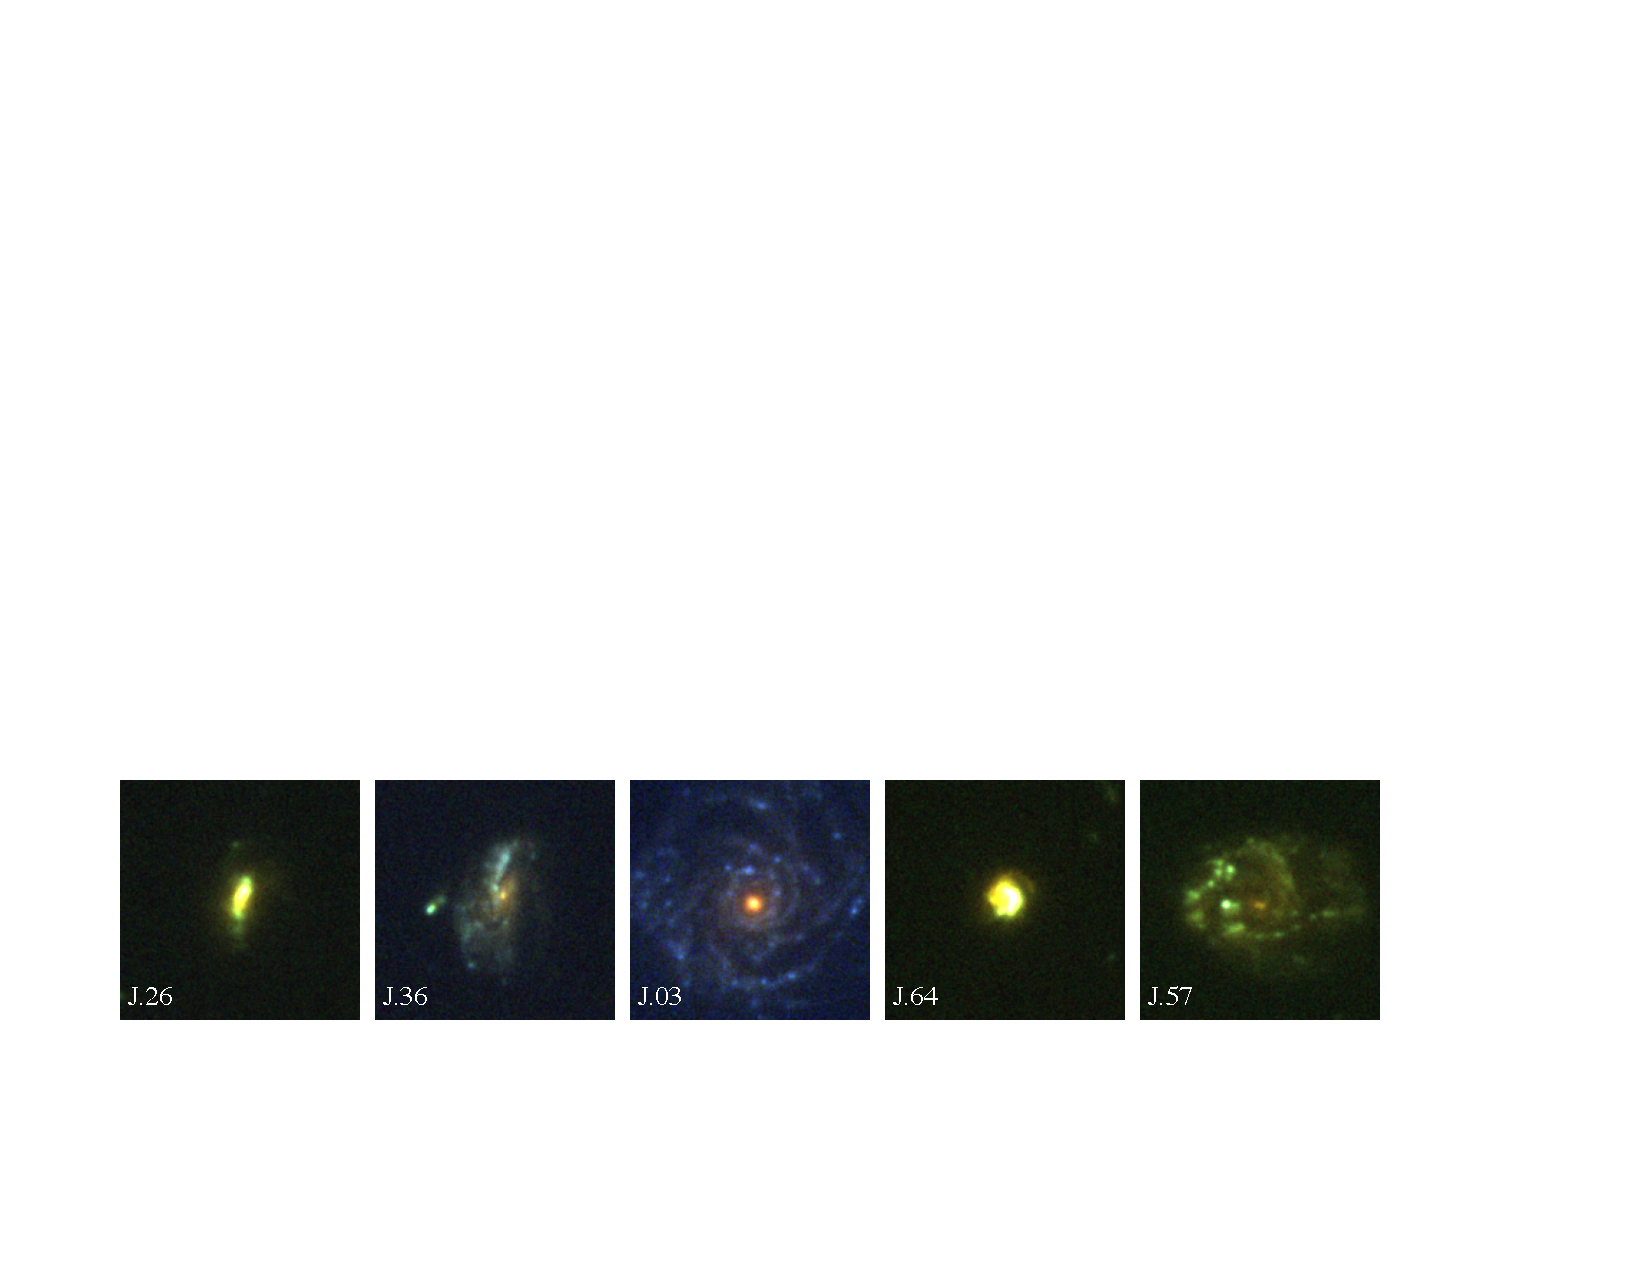
\includegraphics[scale=.75]{../Figures/fors2_color_imstamps.pdf}
\caption{Color imaging of our sample galaxies in the \emph{HST}/ACS F435W, F606W, and F775W filters obtained as part of the GOODS survey (\citeauthor{Giavalisco2004} \citeyear{Giavalisco2004}). Each image is 5\arcsec $\times$ 5\arcsec ( or about $ 35 \rm \ kpc \times 35 \rm \ kpc $) .\label{fig:hstims}}
\end{figure*}

\begin{figure*}[!h]
\centering
\gridline{\fig{../Figures/filt_26_spectra.pdf}{0.5\textwidth}{(a)}
          \fig{../Figures/filt_36_spectra.pdf}{0.5\textwidth}{(b)}}
\gridline{\fig{../Figures/filt_03_spectra.pdf}{0.5\textwidth}{(c)}
          \fig{../Figures/filt_64_spectra.pdf}{0.5\textwidth}{(d)}}
           \fig{../Figures/filt_57_spectra.pdf}{0.5\textwidth}{(e)}
\caption{Keck/LRIS spectra of the sample galaxies and the transmission curves of the filters HeII+47 (blue dashed line) and HeII/3000+48 (red dashed line). The left-hand axis is in units of flux density and the right-hand axis is the percentage of light transmitted by the filter at each wavelength. Vertical dashed lines indicate the wavelengths of the redshifted \ion{Mg}{2}\ doublet. The \ion{Mg}{2}\ doublet falls fortuitously at the central wavelength of the HeII+47 filter for the galaxies shown in panels (a) through (d).}
\label{fig:spec_images}
\end{figure*}

\begin{figure}[h]
\centering
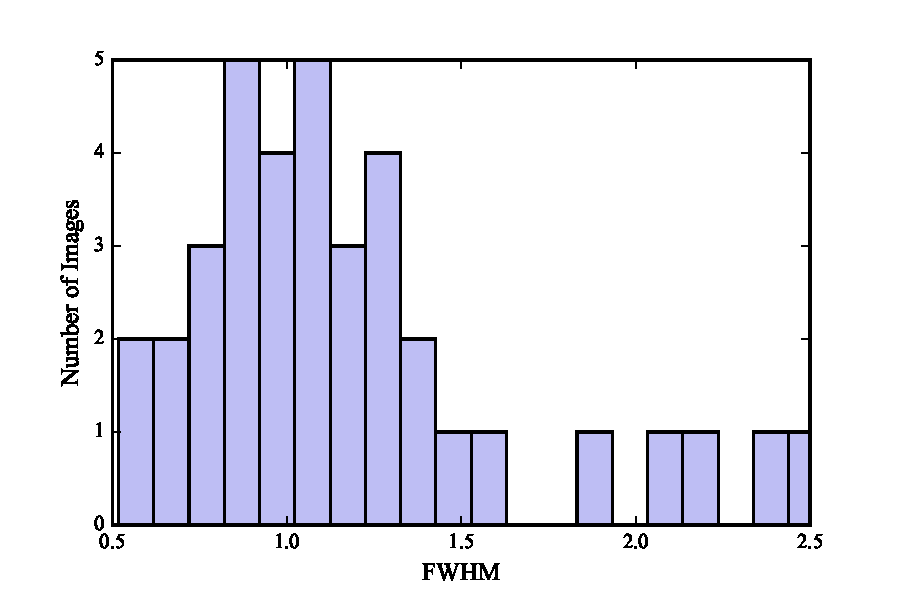
\includegraphics[scale=.55]{../Figures/avg_seeing_HEII.pdf}
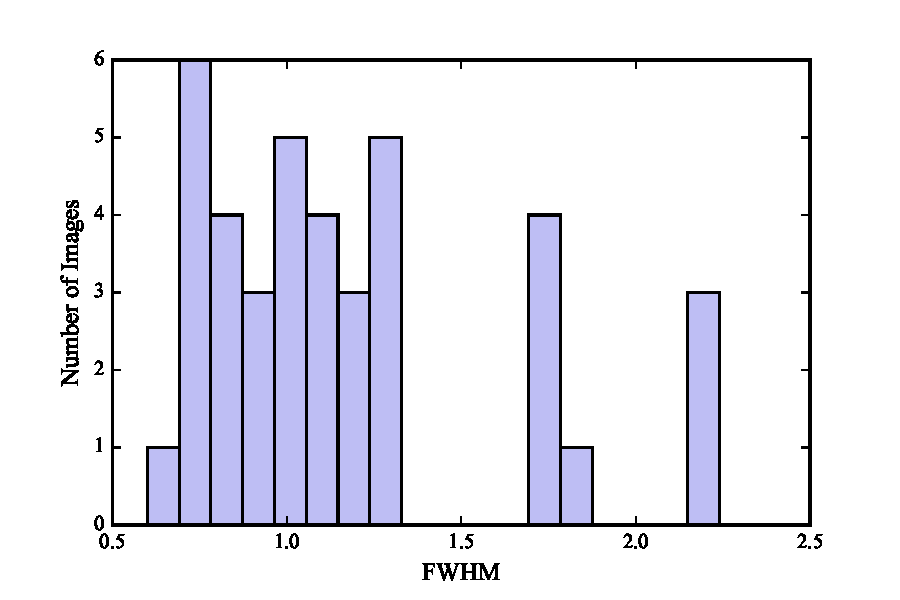
\includegraphics[scale=.55]{../Figures/avg_seeing_HEII3000.pdf}
\caption{\textbf{Top}: Distribution of seeing measurements for the 38 HeII+47 images.
\textbf{Bottom}: Same for the HeII/3000+48 images. The median seeing value for the images in both filters is $\sim 0.8\arcsec$. 
The seeing conditions were calculated from DIMM measurements which are provided by ESO in the header of each science image.
\label{fig.seeing}}
\end{figure}

\subsection{Supplemental Keck/LRIS spectra}
In addition to VLT imaging, in the present analysis we utilize galaxy spectra taken from the \cite{Rubin_2014} Keck I Low Resolution Imaging Spectrometer (LRIS) program.  A $0.9''$ slit width was used for all slitmasks and the median FWHM resolution for the spectra is 274 km s$^{-1}$ at $\lambda_{\rm rest} \approx$ 2800 \AA\ and $286\mkms$  at $\lambda_{\rm rest}\approx$ 2600 \AA\ (see Figure \ref{fig:spec_images}).  The spectral coverage of these data extends from ${\sim}3200$ to 8000 \AA.

\subsection{Image Reduction}
The imaging data were reduced using custom routines written in \emph{Python}. 
The images were first corrected by subtracting and removing the overscan region of the CCD. 
Then the images were bias-subtracted and flat-fielded using twilight flats.
To improve the flat-fielding essential for detecting faint extended emission across the fields, we further correct for the illumination patterns using night-sky flats. The night-sky flats were produced by combining the unregistered science frames with an average sigma-clipping algorithm after masking out all the objects, and any bad pixels. Each individual image was cleaned of cosmic rays and bad pixels by utilizing the \emph{L.A. Cosmic} algorithm \citep{Dokkum2001}.
The astrometry solutions were calculated via Astrometry.net \citep{Lang}, and yield a standard deviation in the galaxy coordinates of $\sigma \approx 0.10''$. Before image stacking, we ran each frame through \emph{SExtractor} \citeth{Bertin} to create a root mean square (RMS) map of each science image.


The final stacked image for each filter is obtained using \emph{SWarp} \citeth{Bertin}.
Each individual frame is first sky-subtracted using a background mesh size of 256 pixels which is approximately $64''$. 
We chose the mesh size to be large enough such that the extended emission is not mistakenly subtracted \citep{Battaia_2015}. 
The frames, after background-subtraction, are resampled onto a common astrometric solution using a \textit{Lancosz3} interpolation kernel. 
The images are weighted by the night-flat image and then  average-combined to increase the signal-to-noise of any \ion{Mg}{2} emission. Additionally, \emph{SWarp} generates stacked RMS images by propagating the error images for each science frame.
Our final stacked images in each filter are shown in Figure~\ref{fig:stacked_image} with the target galaxies indicated.  

\begin{table*}[t]
\centering
\caption{Properties of the 5 galaxies in our sample as estimated in \cite{Rubin_2014}. The EW (in the observed frame) includes both components of the \ion{Mg}{2} doublet and is 
determined from analysis of the supplemental Keck/LRIS spectra.}
\begin{tabular}{llllllll} \hline \hline
Object\footnote{ Name in parenthesis to be used as shorthand for the objects throughout the remainder of the paper. } & R.A. & Dec  & $z$ & SFR($M_{\odot}$ yr$^{-1}$) & $\log{M_{*}/M_{\odot}}$ & EW$_{\rm{obs}}$(\AA) & $\tau_V$\footnote{ Total V-band optical depth of dust as estimated by SED fitting with MAGPHYS. }\smallskip      \\ \hline 
J033225.26-274524.0 (J.26)      & 03:32:25.26 & -27:45:23.9 & 0.6660 & $9.1_{-3.7}^{+1.3}$& $9.86_{-0.04}^{+0.05}$ & $7.539\pm 0.354$ &  $1.227_{-0.20}^{+1.54}$\\ 

J033231.36-274725.0 (J.36)      & 03:32:31.35 & -27:47:24.9 &   0.6669 & $10.5_{-1.6}^{+1.7}$ & $10.02_{-0.03}^{+0.03}$&$5.835 \pm 0.493$ & $1.377_{-0.23}^{+0.60}$\\

J033230.03-274347.3  (J.03)     & 03:32:30.03 & -27:43:47.2  &   0.6679 & $3.8_{-0}^{+0}$ & $10.98_{-0.0}^{+0.01}$ &$12.794 \pm 1.710$ & $0.297_{-0.0}^{+0.0}$ \\

J033229.64-274242.6  (J.64)    & 03:32:29.64 & -27:42:42.5 & 0.6671 & $40.5_{-12.1}^{+8.2}$ & $10.30_{-0.03}^{+0.07}$ &$13.239 \pm 0.263$ & $3.897_{-0.93}^{+1.15}$\\

J033230.57-274518.2  (J.57)    & 03:32:30.56 & -27:45:18.2 &   0.6807  & $12.6_{-2.1}^{+1.7}$ & $10.48_{-0.07}^{+0.03}$ &$6.106 \pm 0.370$ & $1.262_{-0.40}^{+1.23}$ \\

\hline 
\end{tabular}
\label{tab:prop}
\end{table*}

\begin{table}[h!]
\caption{Filter properties  and exposure times of the VLT/FORS2 observations. The width of the transmission curves ($\Delta\lambda$) are calculated by convolving the transmission curve with the total wavelength range of the filter. These values differ slightly from those reported by the European Space Observatory. }
\begin{tabular}{llllll} \hline \hline 
Filter & $\lambda_{\rm{eff}}$(\AA)\footnote{$ \lambda_{\rm{eff}}$ is the effective wavelength of the filter transmission curve.} & $\Delta\lambda$(\text{\AA})    & $N$\footnote{ Total number of images.}   & $T(s)$\footnote{ Total exposure time.} & $S$\footnote{ S, the sensitivity of the filter, is in units of $10^{-17}$ ergs counts$^{-1}$ cm$^{-2}$ .}\smallskip  \\ \hline 
HeII+47  & 4675.21 & 50.11 & 38  & 35,959 & 2.45 \\
HeII/3000+48 & 4722.46  & 44.82 & 38 &   36,937 & 2.40  \\ \hline
\end{tabular}
\label{tab:filters}
\end{table}


\subsection{Absolute Flux Calibration}
We acquired observations of the standard star GD50 from archival ESO calibration imaging at 4 independent epochs. Performing aperture photometry at each epoch and airmass, we calculated the atmospheric extinction coefficients, $k$, to be 0.181 magnitudes for the HeII/3000+48 filter and 0.190 magnitudes for the HeII+47 filter. We perform absolute flux calibration using the methods of \cite{Jacoby1987}. We first convolve the spectral energy distribution of the standard star, $F(\lambda)$ in ergs sec$^{-1}$ \AA$^{-1}$ cm$^{-2}$, with that of the known transmission curve of the filter, $T_{i}(\lambda)$. This yields $F_i$, the total observable flux in each bandpass filter $i$ with units of ergs sec$^{-1}$ cm$^{-2}$:
\begin{equation*}
F_{i}=\int F(\lambda)T_{i}(\lambda)d\lambda.
\end{equation*}
It is not uncommon to assume that $F(\lambda)$ is constant over the small width of the filter. 
%However, our filter transmission curves are sampled at $5$\ \AA\ intervals which is the same sampling as the spectral energy distribution of the standard star obtained from the ESO archives (WILL CHECK CALSPEC). 
However, we calculate the integral numerically.
The system sensitivity, including the defects of the telescope optics and detector response is then given by
\begin{equation*}
S_{i}=\dfrac{F_{i}}{C10^{k_{i}A}},
\end{equation*}\\
where $k_i$ is the extinction in magnitudes per airmass, A is the airmass for each individual exposure, C is the measured count rate of the standard star and $S_i$ is in units of ergs counts$^{-1}$ cm$^{-2}$. Before image co-addition, each science image is corrected for atmospheric extinction by multiplying each frame by $10^{k_{i}A}$. Next, the image is divided by the exposure time, effectively putting the image in units of counts per sec. After co-addition, the images are then multiplied by the appropriate sensitivity factor $S_{i}$. This puts the final images in the appropriate flux units, ergs sec $^{-1}$ cm$^{-2}$.

\begin{figure*}[ht!]
\centering
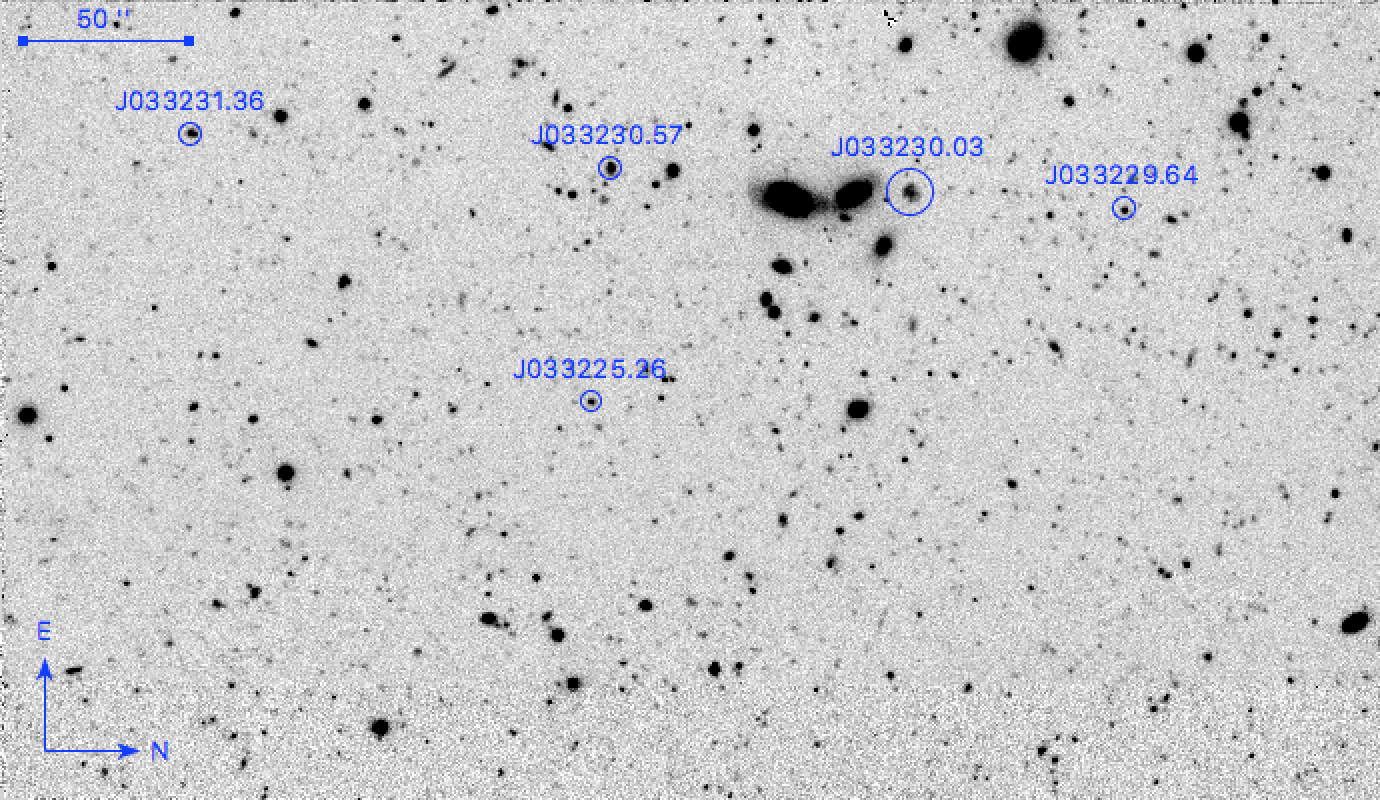
\includegraphics[scale=.61]{../Figures/HEII_final.png}
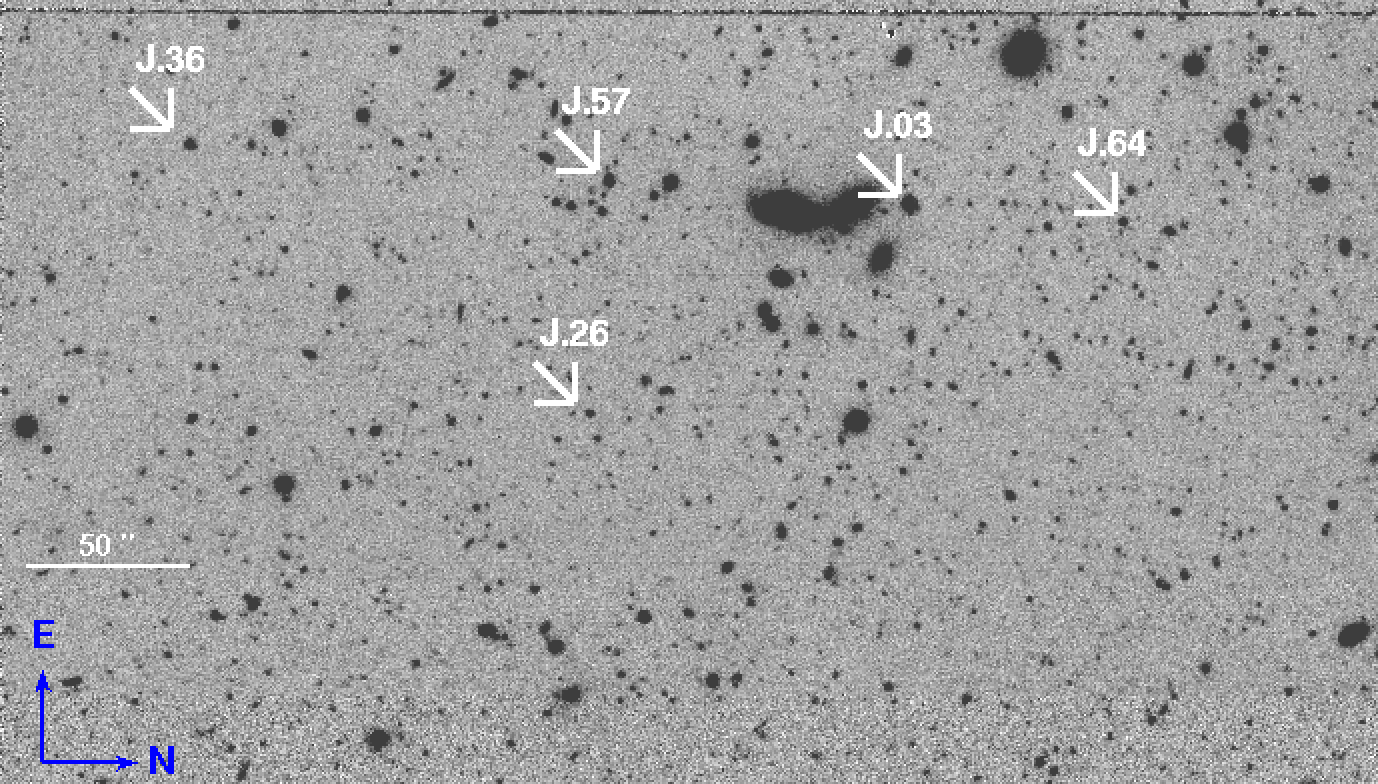
\includegraphics[scale=.61]{../Figures/HEII3000_final.png}
\caption{Top: Stacked HeII+47 image of the galaxy sample. Bottom: Stacked HeII3000+48 image of the same pointing. The exposure time of each image is $\approx 10$ hours. Each image shows half of the total FOV, $5' \times 7'$ which contains the full sample of galaxies (indicated by the white arrows). East is up and North is right.
\label{fig:stacked_image}}
\end{figure*}

\section{Image Subtraction}\label{sec.cont_sub}
We have two goals for our study: (1) assess the surface brightness of line emission in the \ion{Mg}{2} transition in and around each target galaxy; and (2) spatially resolve the morphology of the strong \ion{Mg}{2} absorption observed against the galaxy continua.
To reach both of these goals, we must perform accurate subtraction of the continuum flux of each object from the images taken with the filter covering the targeted line emission. For four of the five galaxies in our sample, the HeII+47 image includes both line and continuum emission, and the HeII3000+48 image provides a high S/N measurement of the continuum only $\approx30$ \AA\ redward of the line emission in the rest-frame. The galaxy excluded from our analysis is J.57. As shown in Figure \ref{fig:spec_images}, the \ion{Mg}{2} transition in this galaxy are equally sampled by both of our filters. When we subtract the continuum image from the \ion{Mg}{2} image we are effectively subtracting the \ion{Mg}{2} continuum. We use this galaxy as check on the quality of our continuum subtraction for reasons.

\subsection{Spectral Correction}
In preparation for continuum subtraction, we first consider whether the continuum level of each galaxy spectrum changes significantly over the passbands of our two filters.
We use the supplementary spectra from \citet{Rubin_2014} to fit the continuum and determine the spectral slope of each galaxy. We use the interactive fitting routine \emph{lt\_continuumfit} from the \emph{linetools} package \citep{Prochaska2016}\footnote{https://github.com/linetools/linetools} to fit the continuum. We then find the total continuum flux in each filter by convolving the fitted continuum with each filter's transmission curve. Next, we take the ratio of both integrated totals, as the ratio will indicate the scaling factor needed to correct our flux measurements prior to continuum subtraction. Comparing these ratios between each galaxy, we find that they are equivalent to within 0.1\%, with a value of 1.118. This value is equal to the ratio between the FWHMs of the filter transmission curves, indicating that spectral slope of each galaxy is approximately flat, and that the continuum level measured in the off-line filter provides an accurate measure of the continuum contribution to the on-line filter flux.

\subsection{Continuum Subtraction}\label{subsec.cont_sub}

To properly continuum-subtract the image taken with the \ion{Mg}{2} filter, we follow a prescription given by \cite{Battaia_2015}. 
We first determine the continuum flux density from the continuum filter,
\begin{equation}
f_{\rm{cont}}=\frac{F_{\rm{cont}}}{\Delta \lambda_{\rm{cont}}},
\end{equation}\\
where $F_{\rm{cont}}$ and $\Delta \lambda_{\rm{cont}}$ are the observed flux per pixel of the continuum image and the transmission FWHM of the continuum filter, respectively. With $f_{\rm cont}$ it is then possible to calculate the flux of any excess emission, $F_{\rm{line}}$:
\begin{equation}
F_{\rm{line}}=F_{\rm{MgII}}-f_{\rm{cont}} \Delta \lambda_{\rm{MgII}}
\label{eq:subtraction}
\end{equation}
where $F_{\rm{MgII}}$ and $\Delta \lambda_{\rm MgII}$ are the observed flux per pixel in the \ion{Mg}{2} filter and the transmission FWHM of the \ion{Mg}{2} filter. The continuum subtracted images of each galaxy are shown in Figure \ref{fig:stamp_images}. The continuum subtracted image has uniform background and no obvious signatures of emission.

\begin{figure*}[!htb]
\centering
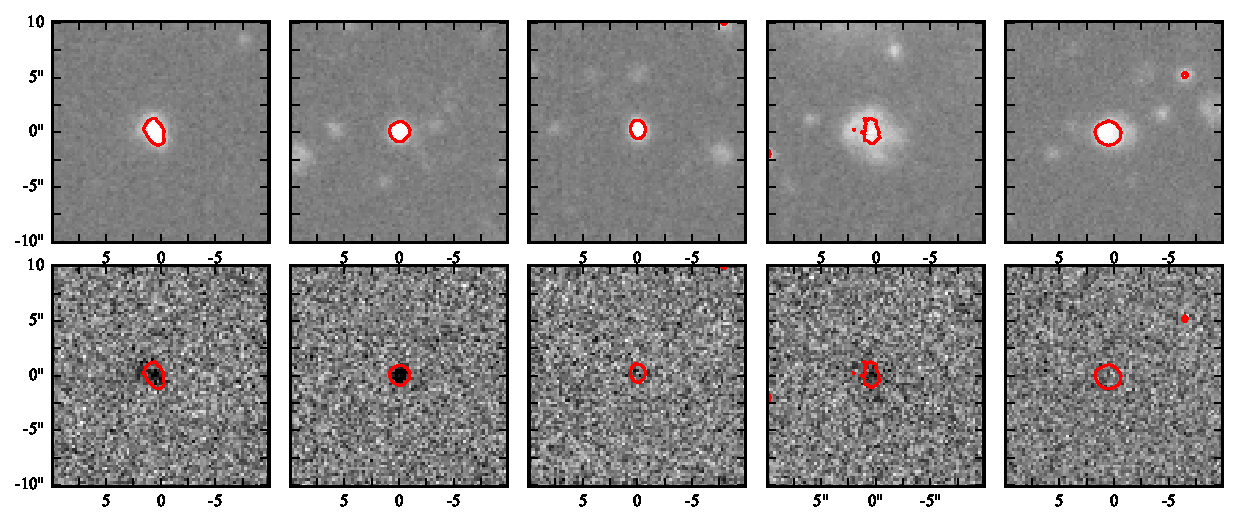
\includegraphics[scale=0.7]{../Figures/stamps.pdf}
\caption{ $10'' \times 10''$ (or about $70 \rm \ kpc \times 70 \rm \ kpc $) images of each galaxy in our sample. Top row: Continuum surface brightness in ergs s$^{-1}$ cm$^{-2}$ arcsec$^{-2}$ measured in the HeII/3000+48 filter. Bottom row: Continuum-subtracted \ion{Mg}{2} surface brightness.  Absorption can be seen in 4 of 5 galaxies. The red contours represent the outline of the 1$\sigma$ surface brightness limit in the HeII+47 image, defined in Sec. \ref{sec.sb}. The colorbar shows the scaling used for the \ion{Mg}{2} images.}
\label{fig:stamp_images}
\end{figure*}

\section{Analysis} \label{sec:analysis}
%   We detail below the resulting surface brightness profiles (Section~\ref{sec.sb}) and detection limits (Section \ref{subsec:test}) as well at the EW$_{\rm{MgII}}$ generated from these data (Section~\ref{subsec.ew}).

\subsection{Surface Brightness Profiles and Limits}\label{sec.sb}
To test for the presence of \ion{Mg}{2} emission, we perform aperture photometry on the continuum subtracted images using the python library \emph{Photutils}. We choose annuli with a radial thickness of 1 pixel or $0.25 ''$, such that $r_{inner}=r_{outer}-1$ (in pixels). Each annulus is centered on the flux-weighted centroid of the galaxy. By dividing the summed flux in each annulus by the area in arcseconds we produce surface brightness (SB) profiles for each galaxy. These profiles are shown in Figure \ref{fig:sb_profiles}. 

\begin{figure*}
\centering
\gridline{\fig{../Figures/J_26.pdf}{0.5\textwidth}{(a)}
          \fig{../Figures/J_36.pdf}{0.5\textwidth}{(b)}}
\gridline{\fig{../Figures/J_03.pdf}{0.5\textwidth}{(c)}
          \fig{../Figures/J_64.pdf}{0.5\textwidth}{(d)}}
           \fig{../Figures/J_57.pdf}{0.5\textwidth}{(e)}
\caption{SB profiles for our sample galaxies. (Top panel) Continuum SB profile (black) measured for each galaxy. The green points show the Mg II + continuum SB measured for the galaxy in the pre-continuum subtracted image. The blue points show the Mg II line SB measured for the galaxy in the continuum subtracted line emission image.  The profile exhibits SB decrements from \ion{Mg}{2} absorption. Photometry was performed in circular annuli. (Bottom panel) The vertical hashes in the bottom show the inner and outer radius of each annulus in kpc. Distance from the center of the galaxy (x-axis) is computed using the average value of the inner and outer radii of each annulus.}
\label{fig:sb_profiles}
\end{figure*}

The error in the SB is determined from the stacked RMS images of each object.  We adopt annuli that are identical to the annuli used to find the SB profiles for each galaxy. To calculate the variance inside each annulus, we sum the RMS pixel values in quadrature, then divide by the area of each annulus. 

To calculate the $1\sigma$ SB limit we follow the procedure of \cite{Battaia_2015}. We first mask out all the sources, their associated extended halos, and edge noise in both the HeII+47 and HeII/3000+48 images. We then calculate the RMS of the background in randomly-placed $1\arcsec$ apertures. We convert these RMS values to SB limits per $1~\rm arcsec^2$  aperture. We find that the 1$\sigma$ detection limits 
(SB$_1$) are $6.332\times10^{-19}$ ergs sec $^{-1}$ cm$^{-2}$ arcsec$^2$ and $5.808\times10^{-19} $ ergs sec $^{-1}$ cm$^{-2}$ arcsec$^2$ in the HeII/3000+48 and HeII+47 filters, respectively. With the 1$\sigma$ detection limit, SB$_1$, determined for the continuum+\ion{Mg}{2} (HeII+47) image, we define a thicker (or ``extended") annulus to be used to search for any extended \ion{Mg}{2} emission. This extended annulus has an inner radius approximately the size of the SB$_1$ isophotal contour for each galaxy. The outer radius is chosen to be the inner radius plus 5 pixels. The mean radii of these extended apertures are 18, 18, 24 and 21 kpc from the centers of the target J.26, J.36, J.03 and J.64 respectively. The resulting SB measurements are shown in Figure~\ref{fig:sb_profiles}.

The sensitivity required to detect an extended source depends on its size, as one can reach lower SB levels by spatially averaging over large apertures. In the ideal case of perfect sky subtraction and continuum subtraction, the 1$\sigma$ SB limit for an extended source is $SB_{1}/\sqrt{A_\text{src}}$, where $A_\text{src}$ is the area in arcsec$^2$ and $SB_{1}$ is the surface brightness limit per 1 arcsec$^2$ aperture. In practice, the actual detection limits are affected by systematics from imperfect subtraction. Therefore, we empirically determine the limits as follows. We mask all the artifacts and sources in the continuum-subtracted images. Next, we generate apertures with sizes similar to our extended annulus ($\sim 20 \rm\ sq.arcsec$), place them at random, and extract the fluxes, $F_{\text{src}}$, within these apertures.

 In the ideal case that the sky and continuum are perfectly subtracted the value of $F_{\text{src}}/ \sigma_{\text{src}}$, where $\sigma_{\text{src}} \equiv SB_{1}\sqrt{A_\text{src}}$, from many random apertures should follow a Gaussian distribution with unit variance. The distribution of $F_{\text{src}}/\sigma_{\text{src}}$ for these apertures is shown in Figure \ref{fig:limits}. We calculate the variance and mean of the distribution and find that the variance of the distribution is $\sigma'_{\text{src}}=1.1$, implying that the SB detection limit for our continuum-subtracted image is higher than $\sigma_{\text{src}}$ by a factor of 10\%. We thus adopt $F_{\text{limit}} \equiv \sigma'_{\text{src}}$  as the $1 \sigma$ upper limit on the total line flux of extended \ion{Mg}{2} emission. The SB$_{\text{limit}}$ is then $F_{\text{limit}}/A_{\rm{src}}$. The values of $F_{\text{src}}$ and 5SB$_{\text{limit}}$ for each galaxy are listed in Table \ref{tab:det_lims}.

\begin{figure}[!ht]
\centering
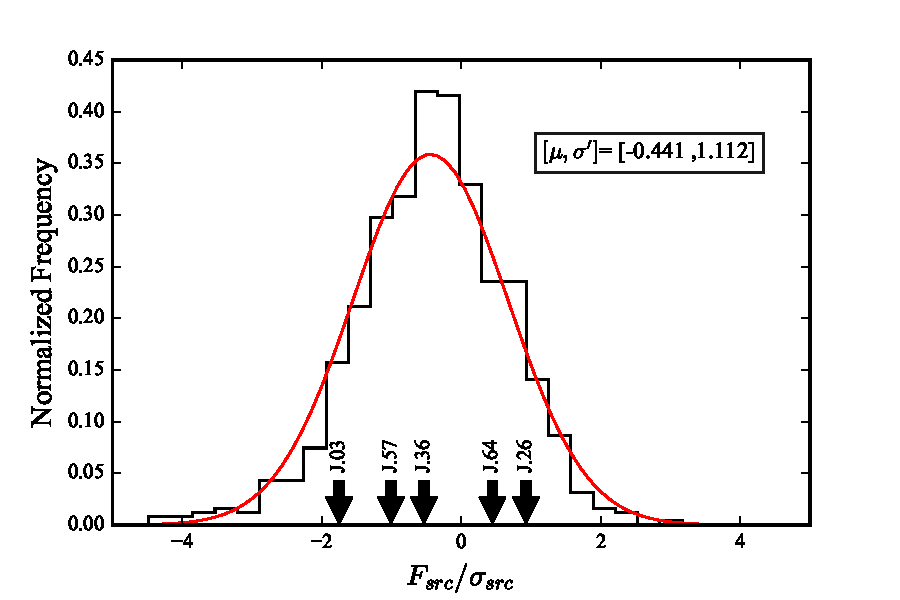
\includegraphics[scale=0.6]{../Figures/hist_sblim.pdf}
\caption{Normalized distribution of $F_{\text{src}}/\sigma_{\text{src}}$ values for random circular annuli placed on the continuum-subtracted line image. $F_{\text{src}}$ is the total flux within an aperture and $\sigma_{\text{src}}$ is the expected $1\sigma$ flux limit in the ideal case of perfect sky and continuum subtraction, i.e $SB_{1}\sqrt{A_\text{src}}$. The black arrows point to the statistical significance of the flux inside the ``extended annulus'' of each galaxy.}
\label{fig:limits}
\end{figure}

\begin{table}[h]
\centering
%\begin{minipage}{4in}
\caption{Significance of extracted flux and detection limits\label{tab:det_lims}}  
\begin{tabular}{lllll} \hline \hline
Object & F$_{\rm{src}}$(\ion{Mg}{2})\footnote{ \ion{Mg}{2} flux is in $10^{-18}$ ergs sec$^{-1}$ cm$^{-2}$. The value in the parenthesis is the statistical significance with respect to $\sigma_{\text{src}}$. } & 5SB$_{\text{limit}}$\footnote{ Limits are in $10^{-19}$ ergs sec $^{-1}$ cm$^{-2}$ arcsec$^{-2}$.} & Area\footnote{ Area of the extended annulus in sq.arcsec.} \\  \hline
J033225.26-274524.0 &  2.44(0.92)& 6.51	& 21 \\
J033232.36-274725.0 &  -1.40(-0.53)& 6.51 & 21 \\
J033230.03-274347.3 &  -5.23(-1.75)& 5.74 & 27 \\
J033229.64-274242.5 &  1.23 (0.44) & 6.22  &26 \\
J033230.57-274518.2 &  -2.53 (-1.00) & 6.81 &18 \\ \hline
\end{tabular}
%\end{minipage}
\end{table}

\subsection{Test of Surface Brightness Limits}\label{subsec:test}
To show that our detection limits are reasonable, we simulate emission with varying intensities. The results of this exercise are shown in Figure \ref{fig:sigmas}. For each galaxy, we assign our simulated emission a constant surface brightness corresponding to 1, 3, 5, 10 and 20 times the $1\sigma$ SB$_{\text{limit}}$ inside the largest annulus used (i.e., the extended annulus). Additionally, we assume Gaussian noise with 1$\sigma$ equal to 1SB$_{\text{limit}}$. After placing the simulated emission around the galaxy, we subtract the continuum in the same manner as explained in Section \ref{subsec.cont_sub}. 

We then construct a smoothed $\chi$ image following the techniques in \cite{Hennawi2013} and \cite{Battaia_2015}. First, we smooth the continuum-subtracted image:

\begin{equation}
I_{\text{smooth}}= \text{CONVOLVE[NB-CONTINUUM]},
\end{equation}
where the CONVOLVE operation indicates convolution of the images with a Gaussian kernel with FWHM=1.5 pixels. Next, we computed the sigma image ($\sigma_{\text{smooth}}$) for the smoothed image ($I_{\text{smooth}}$) by propagating the noise image of the unsmoothed data:
\begin{equation}
\sigma_{\text{smooth}}=\sqrt{\text{CONVOLVE}^2[\sigma^2_{\text{unsmooth}}]},
\end{equation}
where the CONVOLVE$^2$ operation indicates the convolution of the variance image with the square of the Gaussian kernel. The smoothed $\chi$ image is defined by
\begin{equation}
\chi_{\text{smooth}}=\frac{I_{\text{smooth}}}{\sigma_{\text{smooth}}}.
\end{equation}
This $\chi_{\text{smooth}}$ image aids in recognizing the presence of extended \ion{Mg}{2} emission. 

Figure \ref{fig:sigmas} shows the $\chi_{\text{smooth}}$ images for the 5 levels of simulated \ion{Mg}{2} emission. We also include the $\chi_{\text{smooth}}$ image of each galaxy without any simulated emission (in the left most column). The galaxies are outlined by a black isophotal contour corresponding to 1SB$_1$ and the simulated emission is contained inside the extended annulus surrounding each contour. The  $\chi_{\text{smooth}}$ images confirm that we should be able to detect extended \ion{Mg}{2} emission down to a conservative level of 5SB$_{\text{limit}}$. Note again that the SB$_{\text{limit}}$ does indeed take into account the systematics from imperfect continuum subtraction. 


\begin{figure*}[p]
\centering
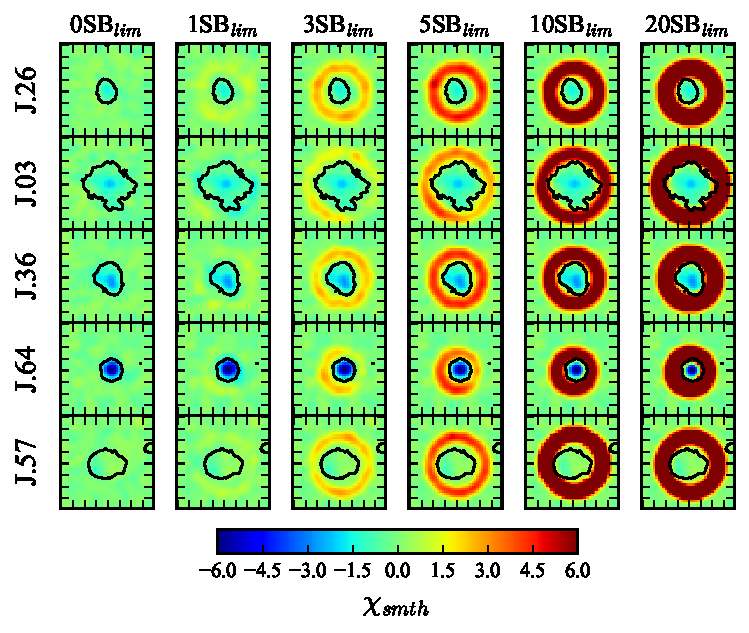
\includegraphics[scale=1.2]{../Figures/sigmas.pdf}
\caption{Continuum-subtracted $\chi_{\text{smooth}}$ images of the 5 galaxies in our sample. Every galaxy is placed in the same row in each column. The columns show simulated emission, with brightness of 0, 1, 3, 5, 10, and 20 times SB$_{\rm lim}$.  Each image has a size of $5'' \times 5''$ (corresponding to $35$ kpc $\times$ $35$ kpc at $z\sim 0.70$). Each image shows the galaxy along with the same isophotal contour used in previous figures (in black).}
\label{fig:sigmas}
\end{figure*}


\subsection{Equivalent Widths}\label{subsec.ew}
Here we derive an expression to calculate the equivalent width (EW$_{\rm{MgII}}$) of any absorption or emission features observed in our narrow-band imaging. Starting from the expression for EW used in the context of spectroscopy,
\begin{equation}
EW_{\lambda}=\int (1-\frac{f_{\lambda}}{f_{\rm{cont}}})d\lambda
\label{eq:specEW}
\end{equation}
we begin by dividing Eq \ref{eq:subtraction} by the flux density of the continuum and the FWHM of the on-line filter,
\begin{equation}
\frac{F_{\lambda}}{f_{\rm{cont}}\Delta \lambda_{\rm{MgII}}}=\frac{F_{\rm{MgII}}}{f_{\rm{cont}}\Delta \lambda_{\rm{MgII}}}- 1.
\end{equation}
Next, we rearrange the above expression such that we produce the argument of the integrand in Eq. \ref{eq:specEW} on the right hand side,
\begin{equation}
-\frac{F_{\lambda}}{f_{\rm{cont}}\Delta \lambda_{\rm{MgII}}}=1-\frac{f_{\rm{MgII}}}{f_{\rm{cont}}}.
\end{equation}
We then approximate the integration in Eq. \ref{eq:specEW} by multiplying the integrand above by the FWHM of the on-line filter $d\lambda=\Delta \lambda_{\rm{MgII}},$
\begin{equation}
-\frac{F_{\lambda}}{f_{\rm{cont}}}=(1-\frac{f_{\rm{MgII}}}{f_{\rm{cont}}})\Delta \lambda_{\rm{MgII}};
\end{equation}
such that
\begin{equation}
EW_{\rm{MgII}}=-\frac{F_{\rm{MgII}}}{f_{\rm{cont}}}.
\end{equation}

Using the above equation along with the continuum and continuum-subtracted images, we produce images of the observed-frame EW$_{\rm{MgII}}$. The observed-frame EW$_{\rm{MgII}}$ images are displayed for each galaxy in Figure \ref{fig:ews} and show only the EWs within the 1$\sigma$ SB$_1$ contours of the corresponding \ion{Mg}{2} images (prior to continuum subtraction). 

\begin{figure*}
\centering
\gridline{\fig{../Figures/J26EW.pdf}{0.8\textwidth}{(a: J.26)}}
 \gridline{\fig{../Figures/J36EW.pdf}{0.8\textwidth}{(b: J.36)}}
\gridline{\fig{../Figures/J03EW.pdf}{0.8\textwidth}{(c: J.03)}}
 \gridline{\fig{../Figures/J64EW.pdf}{0.8\textwidth}{(d: J.64)}}
\caption{Left: Image of the equivalent widths EW$_{\text{\ion{Mg}{2}}}$ inside the red 1SB$_1$ contour. The white contour represents the 0.9\arcsec aperture slit used to measure the equivalent width of absorption in the Keck/LRIS spectrum of each galaxy. Middle: Distribution of  EW$_{\text{\ion{Mg}{2}}}$ values in pixels with continuum flux S/N greater than 1.5 inside the slit aperture. Right: The EW$_{\text{\ion{Mg}{2}}}$ values vs. projected in distance from center are in black and binned EW$_{\text{\ion{Mg}{2}}}$ measurements are shown in red. The horizontal error bars in the radial axis represent the width of the radial bin used.}
\label{fig:ews}
\end{figure*}

To compare our map of EW$_{\text{\ion{Mg}{2}}}$ to the values measured from the Keck/LRIS spectra, we place 0.9 arcsec wide apertures over of each galaxy. The width and position angle of the apertures are consistent with the orientation of the slits used to obtain the spectra. Next, we determine which pixels lie outside the 1$\sigma$ SB$_1$ contours and set their values to zero. Outside this contour, the EW$_{\text{\ion{Mg}{2}}}$ values become poorly constrained due to the lack of S/N in the continuum. We then select all pixels with a S/N $= 1.5$ in the continuum image contour and create a histogram to show the distribution of their EW$_{\text{\ion{Mg}{2}}}$ values. The histograms are shown in Figure \ref{fig:ews}. We also compute the mean equivalent width of these pixels and report their values in Table \ref{tab:abs_props}.
 
To assess the morphology of the \ion{Mg}{2} absorption, we determine the projected distance of each pixel from the center of each galaxy in kiloparsecs. We plot the EW$_{\rm{MgII}}$ vs. this projected distance for each galaxy in the middle panel of Figure \ref{fig:ews}. Although some of the plots suggest a slight upward trend in the values of EW$_{\rm{MgII}}$ with increasing radii, we cannot be confident in this trend because of the large scatter. To better visualize the data and test the significance of the trend, we bin the data radially in 3-5 kpc-wide bins. For example, in Figure \ref{fig:ews}(c), the absorption EW$_{\text{\ion{Mg}{2}}}$ in J.03 extends out to $\sim$ 25 kpc (shown in black in the right-most panel). The EW$_{\rm{MgII}}$ values are binned in 5 kpc increments. We calculate the mean and scatter of the EW$_{\text{\ion{Mg}{2}}}$ in each bin and show these values, in red in the right panels of Figure \ref{fig:ews} and in \ref{fig:ew_comb}.   

\section{Results}\label{sec:results}

\subsection{Limits on \ion{Mg}{2} Emission}
For our sample of galaxies, we are sensitive to extended emission at minimum projected distances of 
18, 18, 24 and 21 kpc from the centers of J.26, J.36, J.03 and J.64 respectively. We do not detect any significant \ion{Mg}{2} emission at these distances around any of our target galaxies. The $\chi_{\text{smooth}}$ images shown in Figure \ref{fig:sigmas} confirm this. A comparison of the simulated emission with the $\chi_{\text{smooth}}$ version of the original continuum-subtracted image, shown in the first column, similarly suggests that we do not detect any extended \ion{Mg}{2} emission. We thus place $5\sigma$ upper limits on the SB of \ion{Mg}{2} emission for each galaxy in the sample, summarized in Table \ref{tab:det_lims}. The most sensitive detection limit using the largest area is SB(\ion{Mg}{2}) = 5.74 $\times$ $10^{-19}$ ergs sec $^{-1}$ cm$^{-2}$ arcsec$^2$, computed for the galaxy J.03. 

\subsection{Spatially Resolved Maps of \ion{Mg}{2} Absorption}
In this section we discuss the details of the absorption detected in our SB profiles as well as compare our EW$_{\rm{MgII}}$ measurements to those measured in the supplemental Keck/LRIS spectra. 

\subsubsection{\ion{Mg}{2}\ Absorption in Surface Brightness Profiles} \label{subsubsec:SBprofiles}
Although we do not detect any extended \ion{Mg}{2} emission, we do observe a decrement of flux, SB$_{\rm abs}$, in the SB profiles of 4 out of 5 galaxies in our sample. As shown in Figure \ref{fig:sb_profiles} absorption from \ion{Mg}{2} ions is prevalent in the profiles between 10 - 25 kpc, decreasing radially outward from the maximum absorption at the center of the galaxies. In Table \ref{tab:abs_props} we report for the galaxies J.26, J.36 and J.03 a maximum decrement in the SB profile due to absorption (SB$_{\rm abs}$) $\sim$ -5 $\times10^{-18}$ erg s$^{-1}$ cm$^{-2}$ per sq.arcsec. Additionally, we report for galaxy J.64 a SB$_{\rm abs}$ one order of magnitude greater with a value of -18.2 $\pm$ 0.127 $\times10^{-18}$ erg s$^{-1}$ cm$^{-2}$ per sq.arcsec. Finally, for J.57, SB$_{\rm abs}$ is strongest at the center of the galaxy with a value of -1.25 $\pm$ 1.115 $\times10^{-18}$ erg s$^{-1}$ cm$^{-2}$ per sq.arcsec. This value is consistent with measuring zero absorption, as expected given the redshift of this system. This measurement suggests that the quality of our subtraction is satisfactory.

\subsubsection{Morphology of MgII Absorption}
Figures \ref{fig:ews}  show the images, distributions and radial projections of \ion{Mg}{2} EWs. We have zeroed out any values that lie outside the SB$_1$ contours for each galaxy. We also impose a signal-to-noise cut, only including EW$_{\text{\ion{Mg}{2}}}$ where the continuum S/N is greater than $1.5$. The mean EW$_{\text{\ion{Mg}{2}}}$ is computed for all pixels inside each Keck/LRIS aperture, defined in Sec. \ref{subsec.ew}, and the resulting values are summarized in Table \ref{tab:abs_props}. Comparing our narrowband EWs with those measured from the spectra, we find agreement to within a 1.6-4.6$\sigma$ for galaxies J.26 and J.36, and more statistically significant differences for galaxies J.03 and J.64. We discuss possible causes for these differences below.

Figure \ref{fig:spec_images}(c) shows the Keck/LRIS spectrum of galaxy J.03. The continuum observed near the \ion{Mg}{2} transition is noisy, compared to the spectra of the rest of the sample. Since the value of the EW$_{\text{\ion{Mg}{2}}}$ is dependent on the level of the continuum present near the \ion{Mg}{2} transition, it may well be that our choice of continuum level in calculating the EW$_{\text{\ion{Mg}{2}}}$ from the spectrum might be higher relative to the continuum level implied by our narrow-band image.


Figure \ref{fig:spec_images}(d) shows the Keck/LRIS spectrum of galaxy J.64. This galaxy is the brightest galaxy in the sample, and also exhibits the highest-velocity wind.  This shifts the \ion{Mg}{2} absorption profile toward the blue end of the 
HeII+47 transmission curve, which could cause the flux in this filter to be weighted toward the continuum level and the absorption signal to be underestimated.

As demonstrated in our radially-binned EW profiles, a majority of the galaxies exhibit large scatter in the binned EW$_{\text{\ion{Mg}{2}}}$ out to larger radii. To better understand the significance of these trends, we construct a plot that compiles the mean EW$_{\text{\ion{Mg}{2}}}$ for all the galaxies, shown in Figure \ref{fig:ew_comb}. To take into account the varying size of the galaxies, we normalize the distances by the approximate radius of the SB$_1$ contour for each galaxy. 

Upon inspection of Figure \ref{fig:ew_comb}, we see that the galaxies exhibit no statistically significant trend in the mean absorption EW as a function of radius inside our 1SB$_1$ isophotal contour, which suggests that the covering fraction is approximately constant across the surface.


\begin{table}[]
\centering
\caption{Properties of \ion{Mg}{2}\ Absorption\label{tab:abs_props}}  
\begin{tabular}{llllll} \hline \hline
Object & SB$_{abs}$\footnote{ Maximum SB decrement, values are in units of $10^{-18}$ ergs sec $^{-1}$ cm$^{-2}$ arcsec$^2$.} & $R$\footnote{ Radius of SB$_1$ contour in kpc.} &\ \ \ EW$_{\text{\ion{Mg}{2}}}^{\rm obs}$($\AA$)\footnote{ Measured from narrowband images, and reported in the observed frame.} & EW$_{\text{\ion{Mg}{2}}}^{\rm obs}$($\AA$)\footnote{ Measured from Keck/LRIS spectra in the observed frame, and includes both lines in the \ion{Mg}{2} doublet.}  \\  \hline
J.26 &  $-5.39 \pm 1.28 $ & 8 &     $\ \ \ 3.51 \pm 0.80$ & $7.53 \pm 0.35 $\\
J.36 &  $-5.64 \pm 0.121 $ & 15 & $\ \ \ 7.69 \pm 1.02$ & $5.83 \pm 0.49$\\
J.03 &  $-4.41 \pm 0.622 $ & 21 & $\ \ \ 5.39 \pm 0.71$ & $12.7 \pm 1.71$\\
J.64 &  $-18.2 \pm 0.127 $ & 10 & $\ \ \ 7.55 \pm 0.66$ & $13.2 \pm 0.26$\\
J.57 &  $-1.25 \pm 1.15   $ & 11& -$0.653 \pm 0.58$ & $6.10 \pm 0.37$\\ \hline
\end{tabular}
\end{table}


\section{Discussion}\label{sec:discussion}
\subsection{Previous Detections of Extended \ion{Mg}{2} Emission}
Previous constraints on the brightness of scattered \ion{Mg}{2} emission were reported by \cite{Rubin_2011}. In this work the authors studied emission from the starburst galaxy TKRS 4389 at $z = 0.69$ with a star formation rate of $49.8\msunperyr$. This emission was detected in a 2-dimensional Keck/LRIS spectrum, with flux from the emission reaching $(8.0 \pm 0.4)$ and $(4.4 \pm 0.4)$ $\times10^{-18}$ ergs sec$^{-1}$ cm$^{-2}$ at  $\lambda _{2796}$ and $(4.0 \pm 0.3)$ and $(2.5 \pm 0.4)$ $\times10^{-18}$ ergs sec$^{-1}$ cm$^{-2}$ at $\lambda_{2803}$ in two independent locations spatially offset from the galaxy continuum. The flux from both emission lines can be converted into two surface brightness values by taking the average of the flux measured at each location and each transition, and dividing by a 1 sq.arcsec aperture. 

Figure \ref{fig:SFR_lim} shows a plot of the 5$\sigma$ detection limits determined for each galaxy in our sample as well as the SB calculated for the galaxy TKRS 4389 vs. SFR. The figure suggests that we should be able to detect scattered \ion{Mg}{2} emission with strengths similar to that detected in TKRS 4389 in our narrowband imaging. Taken at face value, the figure could be consistent with a positive correlation between \ion{Mg}{2} SB and SFR. Future observations are needed to verify this trend, and thus the possibility to detect higher SB of values, as compared to TKRS 4389, \ion{Mg}{2} in emission for high SFR, $>\sim$50 $\msunperyr$. Figure \ref{fig:detection_lim} shows the same SB values as Figure \ref{fig:SFR_lim} vs $\log(M_*/M_{\odot})$. The figure is suggestive that extended \ion{Mg}{2} emission may be brighter in lower mass galaxies. Both \cite{Erb2012} and \cite{Feltre2018} observed a similar trend in their examination of the total \ion{Mg}{2} emission strength vs. galaxy $M_*$.

\begin{figure}[!htb]
\centering
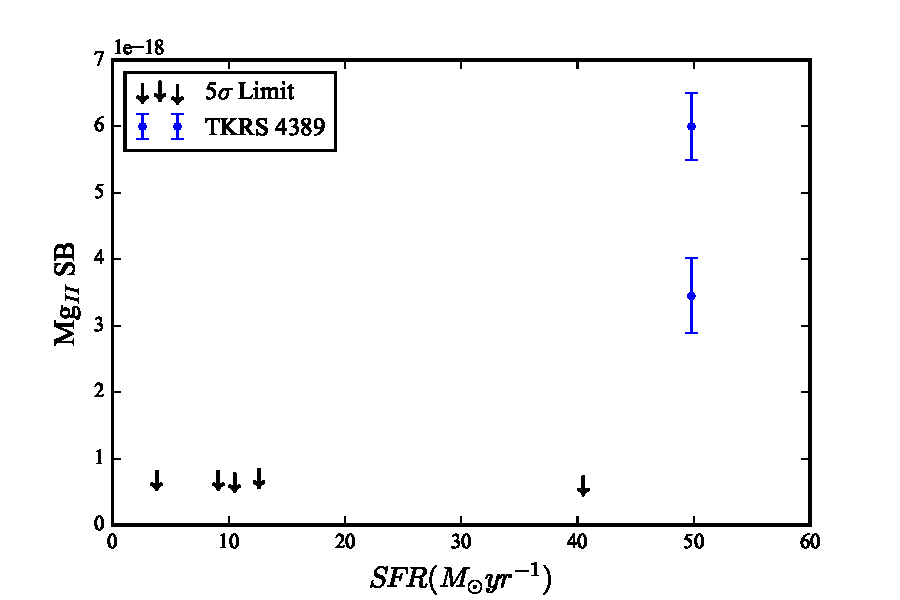
\includegraphics[scale=0.6]{../Figures/limits.pdf}
\caption{Comparison of our detection limits to the measured extended emission of TKRS 4389 vs SFR. The arrow color-galaxy scheme is: The blue arrow indicates J.26, green indicates J.36, red indicates J.03, and cyan marks J.64. Our imaging is sufficiently sensitive to detect extended emission at similar strengths to the extended emission measured for TKRS 4389 with SFR $\sim 50 \msunperyr$.}
\label{fig:SFR_lim}
\end{figure}

\begin{figure}[!htb]
\centering
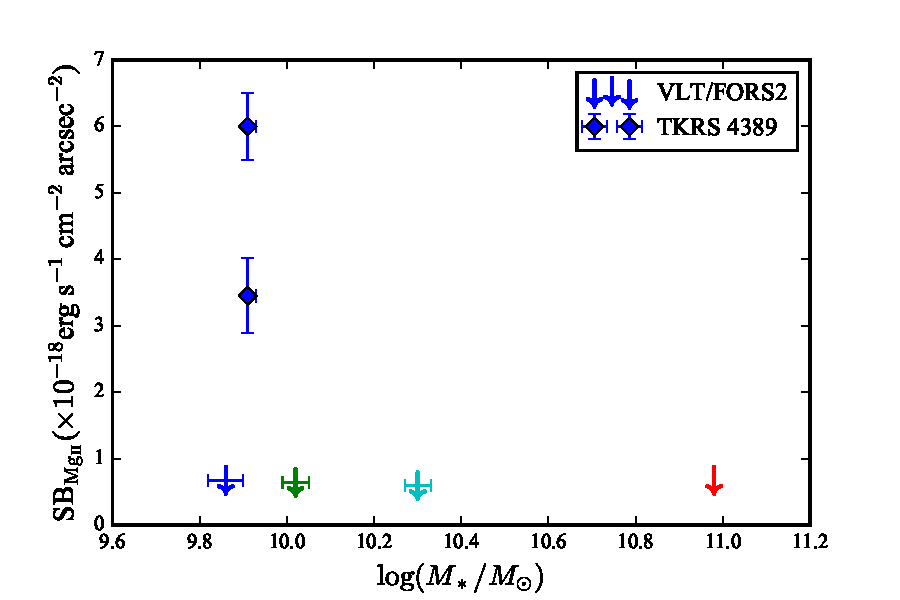
\includegraphics[scale=0.6]{../Figures/mass_limits.pdf}
\caption{Comparison of our detection limits to the measured extended emission of TKRS 4389 vs Stellar Mass. The color scheme is the same as Figure \ref{fig:SFR_lim}.}
\label{fig:detection_lim}
\end{figure}

\subsection{Geometry of Scattering Material}
In the context of the idealized models of cool gas outflows, discussed in \cite{Prochaska_2011}, radiative transfer calculations predict that strong \ion{Mg}{2} emission is generated along with ubiquitous blueshifted absorption of \ion{Mg}{2}. For isotropic and dust-free scenarios, photons are conserved, as any absorbed continuum photon is eventually re-emitted.  Therefore, the total equivalent width of both the absorption and emission features is equal to zero in such models. Assuming that our galaxies host an isotropic and dust-free wind, we wish to determine how much emission is predicted to be generated by this wind, and how the SB of this emission compares to our detection limits.

To calculate the predicted emission flux we first determine the flux absorbed by \ion{Mg}{2} ions. Using our Keck/LRIS spectra, we find the average value of the continuum near the \ion{Mg}{2} doublet and multiply this value by the observed EW of the doublet. Then to estimate the SB, we distribute this flux uniformly inside multiple annuli of varying sizes. These annuli all have an inner radius equal to the galaxy's isophotal radius and successively larger outer radii.  Additionally, since our SB limits are dependent on the size of the aperture used, we calculate the SB detection limits of our images inside each of the aforementioned annuli. Figure \ref{fig.emission} shows how the SB of emission varies with the spatial extent of the annulus (red hexagons), as well as how the SB compares with our detection limits (thin black curve). Except for the case of galaxy J.03, the SB of this ``missing'' emission lies above our detection limits. 
Under the assumption that the wind in these galaxies does in fact extend beyond the $\rm SB_1$ isophotal contour (at $R = 8-21$ kpc), this result suggests that these galaxies do not host isotropic, dust-free winds.  

\subsubsection{Anisotropic, Dust Free Winds}

There are many phenomena that may reduce the SB of the scattered \ion{Mg}{2} emission so that it is consistent with our observations. One factor that can affect the observed emission strength is the morphology of the wind. Anisotropic winds were shown in \cite{Prochaska_2011} to exhibit reduced emission strengths compared to isotropic winds. Direct evidence of anisotropic winds, and specifically of a bipolar morphology, has been observed in emission from cold and shock-heated gas around local starburst galaxies \citep[e.g.][]{{Walter2002,Westmoquette2008M,Strickland2009}}. For distant galaxies, enhanced \ion{Mg}{2} absorption along a galaxy's minor axis \citep[][]{{Bordoloi2011,Kacprzak2012,Bouche2012}} observed along background QSO sightlines, are suggestive of bipolar outflows. Furthermore, \cite{Rubin_2014} analysis demonstrating a strong dependence of incidence of winds observed via blueshifted absorption on galaxy orientation is suggestive of the ubiquity of bipolar outflows in distant galaxies.

We now assume that the brightness of emission in our galaxies is reduced by the effect of anisotropy. For the anisotropic winds modeled in \cite{Prochaska_2011}, the emission is reduced by the factor $\Omega/4\pi$, where $\Omega$ is the angular extent of the wind. As \citet{Prochaska_2011} points out, given that the outflow must cover most of the continuum in order to be detected, the value of $\Omega$ has an approximate lower limit of $\Omega > 2\pi$. We show the predicted SB profiles for wind emission from our galaxies assuming  $\Omega = 2\pi$ with gray diamonds in Figure  \ref{fig.emission}.

After reducing the SB of the expected \ion{Mg}{2} emission by the corresponding factor of 2, we predict profiles that fall below our SB detection limits for galaxies J.26 and J.36. However, the SB profile of J.64 remains above our SB detection limits, suggesting additional phenomena are needed to reduce the strength of scattered emission. Previously discussed in Section \ref{sec:results}, this object is the intrinsically brightest galaxy in our sample and exhibits the strongest \ion{Mg}{2} absorption, which suggests the presence of a strong ISM component. \cite{Prochaska_2011} note that \ion{Mg}{2} photons can be more effectively trapped in objects with a large amount of dusty interstellar material. 

\subsubsection{Anisotropic, Dusty Winds}

Dust in the wind is another factor that can reduce the observed emission strength, and affect the shape of the line profile. 
In the \cite{Prochaska_2011} models that include dust in the wind material, the dominant effect is that the most redshifted emission is suppressed. The line flux is reduced by a factor of $(1+\tau_{\rm{dust}})^{-1}$, where $\tau_{\rm{dust}}$ is the integrated opacity of dust. Estimates of the dust content, assuming that the wind has the same dust content as the ISM, of each galaxy come from the SED modeling performed \cite{Rubin_2014}, and are shown in Table \ref{tab:prop}. The blue triangles in Figure \ref{fig.emission} show the predicted SBs for an anisotropic wind with dust. For the galaxies J.26, J.36 and J.03, the introduction of dust reduces the predicted emission further below our detection limits. For galaxy J.64, in which anisotropy alone did not reduce the predicted emission of J.64 below our detection limits, Figure \ref{fig.emission} shows that a combination of dust and anisotropy is sufficient to reduce the strength of the scattered emission of J.64 below our detection limits. 


\section{CONCLUSION}\label{sec:conclusion}
We have presented the results of a narrowband imaging search for \ion{Mg}{2} emission around a sample of star-forming galaxies at a redshift of $z \sim 0.70$ which are known to exhibit outflows traced in \ion{Mg}{2} absorption. We did not detect any \ion{Mg}{2} emission in this sample, and place a $5\sigma$ detection upper limit on the surface brightness of SB(\ion{Mg}{2}) $\approx$ 5.74 $\times 10^{-19}$ ergs sec $^{-1}$ cm$^{-2}$ arcsec$^2$. This limi is determined within annuli with areas of , $\sim 20$ sq.arcsec, and having mean radii of 13, 18, 21 and 24 kpc from the centers of each target. Our imaging also spatially resolves the strength of the \ion{Mg}{2} absorption observed against the galaxy continua yielding novel information of the \ion{Mg}{2} absorption morphology. This absorption fully covers the galaxies from their centers out to isophotal radii defined by the SB$_1$ (1$\sigma$) depth of a continuum + \ion{Mg}{2} image (at approximately $\sim 22$ kpc), suggesting that the absorbing gas is optically thick and completely covers the stellar disks out to this distance. Additionally, radial projections of the mean EW measured for our sample galaxies suggest that the EWs due to \ion{Mg}{2} are approximately constant across the galaxies surfaces. 

We compared our surface brightness detection limits with the prediction of the radiative transfer models of \cite{Prochaska_2011}. We are able to rule out that the winds in our sample are isotropic and dust free, as our images are sufficiently sensitive to detect the emission predicted by such models. Adopting the assumption of dusty and/or anisotropic winds, reduces the strength of the predicted \ion{Mg}{2} emission to lie below our detection limits.  Although these limits suggest that the winds in our sample are not isotropic and dust-free, questions linger regarding the relative roles wind anisotropy, dust content, and extent play in reducing scattered emission. Thus, deeper imaging or spatially-resoled spectroscopy of \ion{Mg}{2} is will be needed to fully characterize the morphology of these winds. 




\begin{figure*}[!htb]
\centering
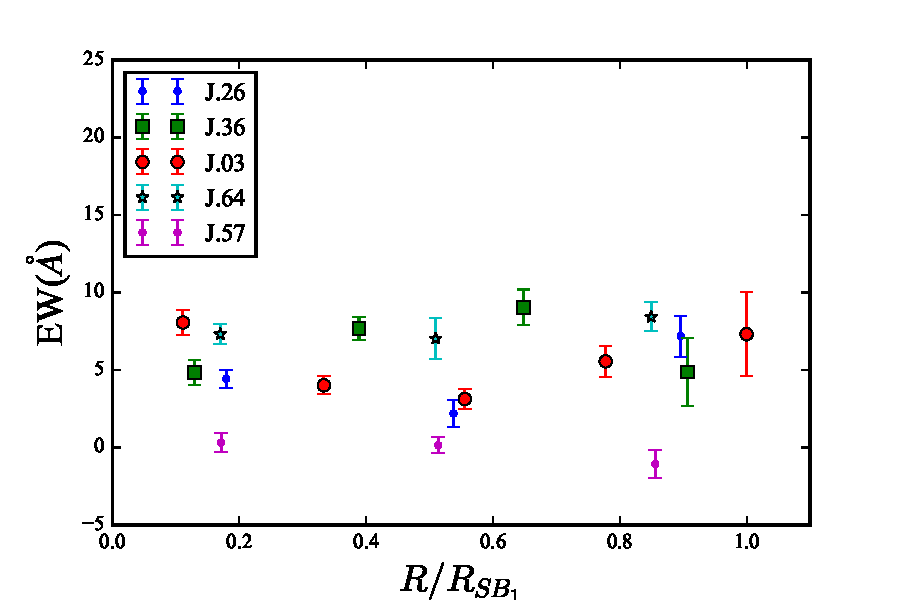
\includegraphics[scale=0.9]{../Figures/ew_comb.pdf}
\caption{Radial profile of the mean EW of \ion{Mg}{2} absorption for all galaxies. The mean EW values are the same as those shown in the right column of Figure \ref{fig:ews}. We have normalized the corresponding radii by the approximate size of the SB$_1$ contour of each galacy. There is significant scatter relative to the error bars at extended distances.}
\label{fig:ew_comb}
\end{figure*}

\begin{figure*}[h]
\centering
\gridline{\fig{../Figures/geo_J26.pdf}{0.5\textwidth}{(a)}
          \fig{../Figures/geo_J36.pdf}{0.5\textwidth}{(b)}}
\gridline{\fig{../Figures/geo_J03.pdf}{0.5\textwidth}{(c)}
          \fig{../Figures/geo_J64.pdf}{0.5\textwidth}{(d)}}
\caption{Predicted SB of \ion{Mg}{2} emission for isotropic and anisotropic dust-free winds. The red hexagons show the expected SB of emission that has been uniformly distributed inside an annulus (with inner radius equal to the radius to that of the galaxy's isophotal radius and an outer radius equal to the x-axis value) for an isotropic wind. The gray diamond points show the SB of \ion{Mg}{2} emission for withs with angular extent $\Omega=2\pi$, or an anisotropic wind. The blue triangles mark the predicted SB for a wind that is anisotropic and affected by dust. The solid line shows the value of our SB detection limits. The dashed vertical and horizontal lines represent the outer radius of the extended annulus used to measure the initial detection limits and the value of the SB detection limit in that annulus. The legend in panel (a) holds for the remaining panels.}
\label{fig.emission}
\end{figure*}



\bibliography{references2017}

\end{document}